\documentclass[12pt, a4paper, onecolumn]{article}
\usepackage{fontspec}
\usepackage{titlesec}
\usepackage[english]{babel}
\usepackage{blindtext}
\usepackage[demo]{graphicx}
\usepackage{subfig}
\usepackage{pgf}

\setmainfont{Georgia}
\titleformat{\section}
{\normalfont\fontspec{Arial}\fontsize{20pt}{0}\bfseries}
{\thesection}{20pt}{}

\begin{document}

\paragraph{Accidents related to falling} is a major issue in our society. In fact, according to the World Health Organization, "Falls are the second leading cause of accidental or unintentional injury deaths worldwide" \cite{who}. Globally, an average of 37.3 million people (Jan 2018) suffer from injuries related to a fall each year, which are severe enough to seek medical attention. Out of these, no less than an estimated 640 000 individuals die as a direct consequence of the fall \cite{who}. Fall  related accidents are therefore to be considered as a significant world wide health problem. 

\paragraph{Although Age} is identified as a key driving factor behind fall related injuries, it is not by far the only reason that people hurt them selves this way every year.  Other risk factors include 
	\begin{itemize}
		\item Occupations which require you to work at an elevated height.
		\item Alcohol and substance abuse.
		\item Medical conditions contributing to a reduced sense of balance or vision.
		\item Sporting.	
	\end{itemize}

\paragraph{In Sweden} alone, statistics shows even darker figures. Here, falling is the single one reason responsible for the greatest number of accident related fatalities, hospitalizations, and visits to emergency clinics, outnumbering traffic accidents, who come in second \cite[p~3,5]{msb_report}. On top of that, in Sweden, falling is together with poisoning, the type of accident who poses the biggest annual growth, having duplicated the amount of yearly incidents since 2000 \cite{soc_olyckor} Studies have also showed that peoples perception target traffic accidents as the the most common cause of the above \cite[p~5]{msb_report}. That is however not true, but a reasonable explanation for this is according to MSB (Swedish Civil Contingencies Agency) that most fall related accidents happen in a domestic area and are thus not as dramatic as a car accident or a fire for example. This tend to give this type of accident less space in the common media. 

\paragraph{}The work force is by no means an exception to the statistics presented above in Sweden .The swedish work environment authority (Arbetsmiljöverket) published a study in 2016, claiming that fall accidents are the most versus second most common reason for absence in work due to accident, for women and men respectively \cite[p~1]{av}. This does not only have an impact on the lives of the individual and his or her family, it also poses serious economical damage to the society in general, and the affected organizations in particular. The diagram below illustrated the amount of fall related accidents in the most affected occupations. 


\begin{figure}[h]
	\centering
	\subfloat[label 1]{{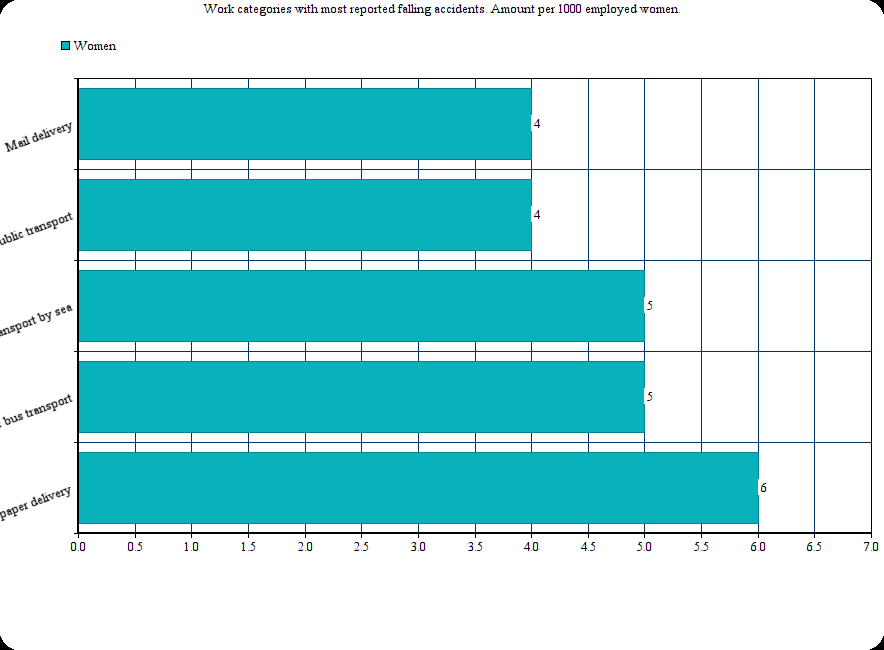
\includegraphics[width=6cm]{../img/Fall_from_ground_women.png} }}%
	\qquad
	\subfloat[label 2]{{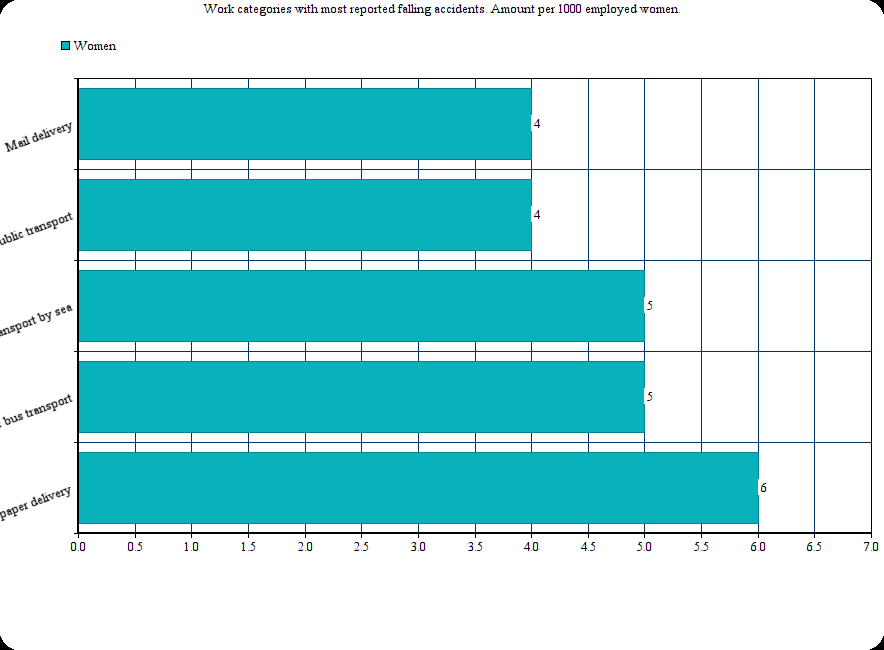
\includegraphics[width=6cm]{../img/Fall_from_ground_women.png} }}%
	\caption{Män och kvinnor som faller från stående höjd}%
	\label{fig:example}%
\end{figure}

\begin{figure}[h]
	\centering
	\subfloat[label 1]{{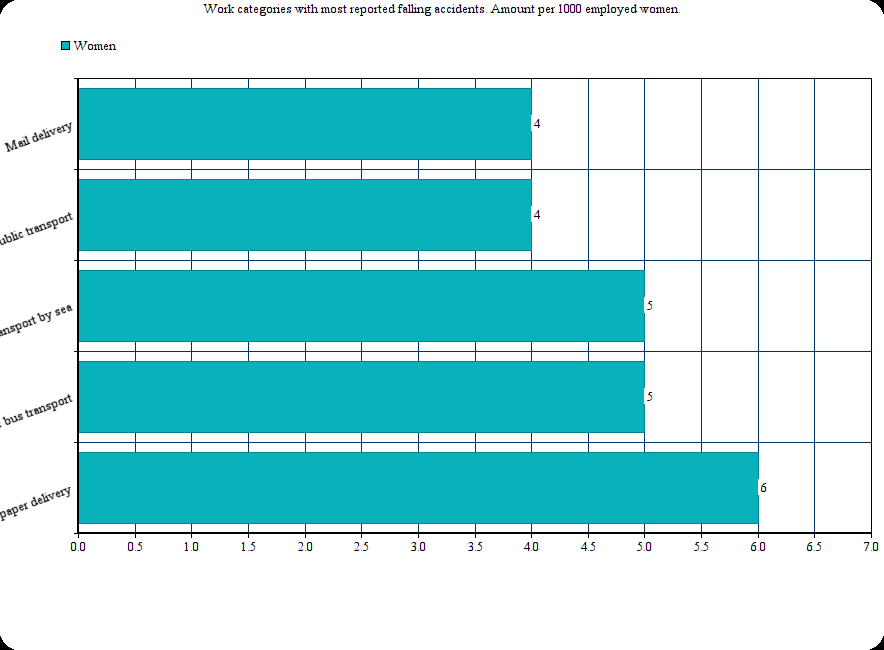
\includegraphics[width=6cm]{../img/Fall_from_ground_women.png} }}%
	\qquad
	\subfloat[label 2]{{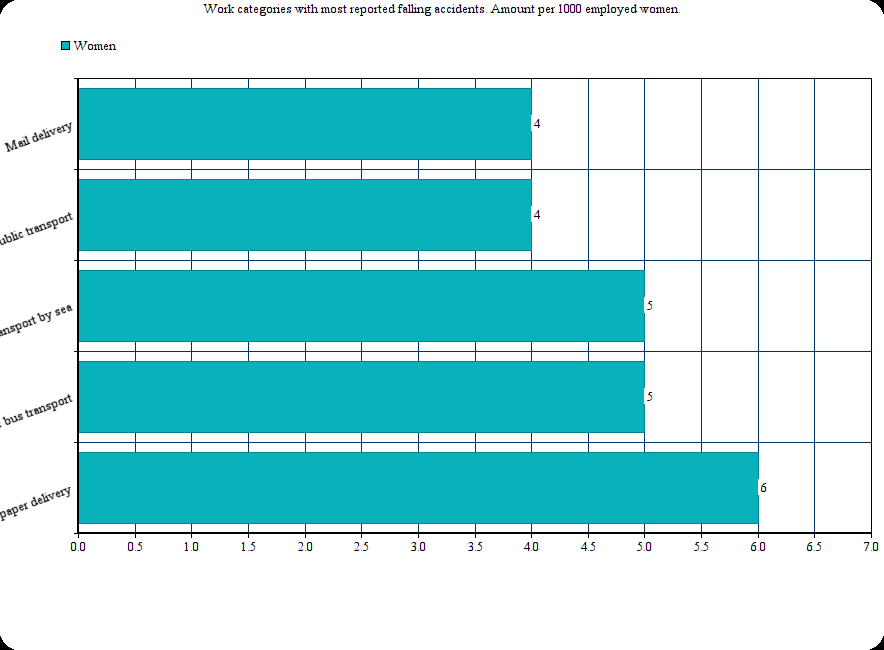
\includegraphics[width=6cm]{../img/Fall_from_ground_women.png} }}%
	\caption{Män och kvinnor som faller från eleverad höjd}%
	\label{fig:example}%
\end{figure}



\bibliography{bib_peter}
\bibliographystyle{ieeetr}

\end{document}